\documentclass{article}
\usepackage[a4paper, total={6in, 8in}]{geometry}
\usepackage{graphicx}
\usepackage{hyperref}
\usepackage{subcaption}
\usepackage{tabularx}
\begin{document}

\date{04/2024}

\title{\Large \bf Report: communcation jitter analysis, periodic peaks}

\author{Davide Rovelli, Michele Dalle Rive}
\maketitle

\section{Objective}
We analyse the latency disitribution in the communication between 2 bare-metal 
nodes in a datacenter. The objective of our experiments is to make packet 
processing latency of Linux-based hosts with modern NICs as \textit{deterministic}
as possible. This consists in reducing communication jitter to a minimum, where
$jitter = \max(latency) - \min(latency)$.

Contrarily to usual low tail-latency experiments/systems which aim to reduce the
common-case latency up to some percentile (e.g.$99.5\%, 99.9\%$) we want to minimise 
the $100\%$ latency, even at the cost of (non-substantially) increasing the 
common-case. 

\section{Methodology}

\subsection{Benchmark}
\label{sec:benchmark}
We run ping-pong tests across 2 hosts \textbf{A} and \textbf{B} by sending packets
at a fixed sending rate. Each packet carries a packet ID and 4 timestamps:

\begin{itemize}
  \itemsep=-0.8mm
  \item $ts_1$: timestamp just before sending the PING message in host \textbf{A}
  \item $ts_2$: timestamp as soon as the process in host \textbf{B} receives the
  PING packet.
  \item $ts_3$: timestamp just before sending the PONG message in host \textbf{B}
  \item $ts_4$: timestamp as soon as the process in host \textbf{A} receives the
  PONG packet.
\end{itemize}

We then calculate the difference between timestamps of successive packets
to get the variations in jitter. For example, $ts_1(33) - ts_1(32)$ where 33 and
32 are the packet IDs, represents the time interval between the PING send timestamp
of packet 32 and the PING send timestamp of packet 33. If there's no jitter,
it should be equal to the sending rate. The difference between $ts_1(33) - ts_1(32)$
and the sending rate represents the relative jitter for that pair. 

\subsection{Hardware setup}
2x CloudLab xl170 nodes. See \href{cloudlab.us}{cloudlab.us}
for more detailed specs.

\begin{itemize}
  \itemsep=-0.8mm
  \item CPU:  Intel Xeon E5-2640 v4 at 2.40GHz, 10 cores, 64GB RAM
  \item OS/kernel: Ubuntu 22.04.4 LTS / 6.6.19-060619-generic x86\_64
  \item NIC/driver: Mellanox Connect-X 4 / mlx5 
\end{itemize}

% \paragraph{Cluster B} 2x internal cluster nodes: 

% \begin{itemize}
%   \itemsep=-0.8mm
%   \item CPU:  Intel Xeon E5-2680 v4 at 2.40GHz , 28 cores, 64GB RAM
%   \item OS/kernel: Ubuntu 22.04.4 LTS / 6.6.19-060619-generic x86\_64
%   \item NIC/driver: Mellanox Connect-X 4 / mlx5 
% \end{itemize}


Nodes are connected over Ethernet, the physical connection is likely to span multiple
switches. No concurrent traffic should be present as CloudLab guaranteed 
experiment reproducibility.

\subsection{Software setup}
\label{sec:software}
We use different \textit{kernel bypass} methods in order to minimize the 
well-known overhead introduced by the classical network stack in Linux machines.
We test the following: 

\begin{itemize}
  \vspace{-0.8mm}
  \itemsep=-0.4mm
  \item RoCE, specifically double-sided SEND/RECV RDMA with the Unreliable Datagram (UD) 
  transport type
  \item eBPF XDP in two different modalities:
  \vspace{-1.8mm}
  \begin{itemize}
    \itemsep=-0.5mm
    \item XDP offload: packet is handled by an eBPF XDP hook and executed as early
    as possible in the network stack. 
    \item AF\_XDP: XDP socket type which pushes the TX and RX buffer management to 
    the application level.
  \end{itemize}
    \item Standard network stack over UDP    
\end{itemize}

\noindent
Packet size: \textit{1024 bytes}


\section{Analysis of periodic outliers}
Here we show some of the results which include interestingly periodic latency 
outliers, which we refer to as ``peaks''. We observe two types of periodic peaks 
of which we have not yet identified the root
cause. We refer to them as \textbf{$ts_1$-offset} and \textbf{$ts_2$-arrow}.

\autoref{fig:1} shows a typical benchmark with a thick baseline around the 
sending rate ($996\mu s$), which means that most packets are subject to a minimal 
jitter, and the outliers that we analyze below.

\paragraph*{$ts_1$-offset} The top-left plot in \autoref{fig:1}, representing the difference
between 2 successive send events of the PING packet on host A, shows 
\textbf{$ts_1$-offset}:
a small number of outliers delayed from baseline by a similar offset in the 
y-axis ($\approx150\mu s$). Successive outliers evenly spaced, meaning there is a 
fixed number of packet (i.e. time interval) between them. 

\paragraph*{$ts_2$-arrow} The top-right plot in \autoref{fig:1}, representing 
the difference 
between 2 successive receive events of the PING packet on host B, shows 
\textbf{$ts_2$-arrow}: a 
series of outliers with decreasing amplitude. Every outlier on top of the 
baseline (delayed packet) is immediately followed by a symmetric point below the
baseline which shows that the successive packet was not delayed, hence the 
difference between its timestamp and the one of the previous delayed packet is
less than then sending rate. 
Successive outliers forming the arrow are evenly spaced, meaning there is a 
fixed number of packet (i.e. time interval) between them. 


\paragraph*{} Bottom left and bottom right plot show no periodic outliers, 
meaning that the PONG send and receive events do not seem to be subject to
periodic peaks in our experiments. \textbf{$ts_1$-offset} and 
\textbf{$ts_2$-arrow} have the following characteristics:

\begin{itemize}
  \item Independent from the software technology used, they manifiest with all 
  bypass techniques listed in \autoref{sec:software} as well as the normal 
  network stack. 
  \item Throughput dependent: changing the sending rate changes some 
  characteristics as we cover in \autoref{sec:sending_rate}
  \item Partially deterministic: 2 runs with the same settings often leads to 
  the same result but not always, especially \textbf{$ts_2$-arrow} seems to be
  the most variable. 
  \item The total amount of outliers of both types is less than the 0.01\% and
  decreases even further when isolation techniques are applied.
\end{itemize}



\begin{figure}
  \centering
  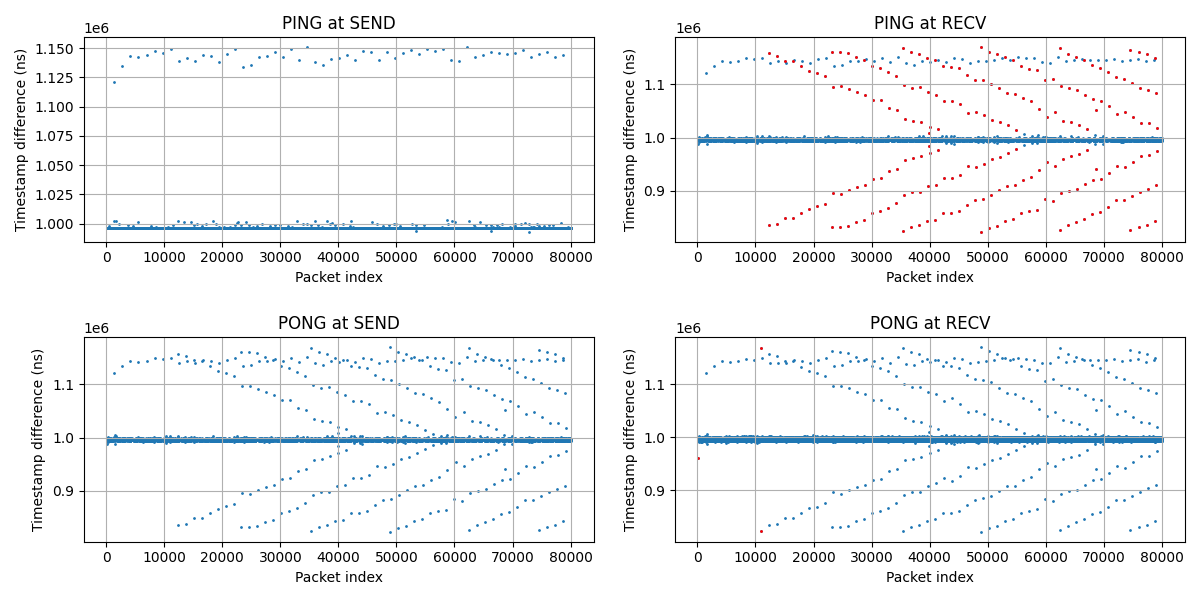
\includegraphics[width=\textwidth]{fig/xsk_80k_996us_powermax.png}
  \caption{Pingpong benchmark plot - sending interval $996\mu s$. Each dot corresponds 
  to a packet ID (x-axis) and the difference between its timestamp and the timestamp 
  of the packet with the previous ID (y-axis). The sending interval is fixed and 
  packets are sent in order. See \autoref{sec:benchmark} for a more detailed
  explanation of the benchmark}
  \label{fig:1}
\end{figure}


\subsection{Effect of sending rate}
\label{sec:sending_rate}

The sending rate of the PING packet seems to affect both \textbf{$ts_1$-offset} 
and \textbf{$ts_2$-arrow}. 

\autoref{fig:interval_variations} shows 5 different 
tests in which we can see the density, offset and shape of the two periodic 
outliers types change. \autoref{fig:999us}, \autoref{fig:1000us}, 
\autoref{fig:1001us} have sending periods of respectively $999\mu s, 1000\mu s$
and $1001\mu s$, which result in quite noticeable differences in the latency
plots. We can observe that \textbf{$ts_1$-offset} (left plot) changes in terms
of density and offset, respectively of $\approx90\mu s$, $\approx160\mu s$ 
and $\approx50\mu s$. \textbf{$ts_2$-arrow} also varies in angle, density and 
periodicity. The 2 bottom plots \autoref{fig:200us} and \autoref{fig:50us} show 
results with sending periods of respectively $200\mu s$ and $50\mu s$. Here 
\textbf{$ts_2$-arrow} is replaced by a ``line'' which is similar to 
\textbf{$ts_1$-offset}. This characteristic was often observed in sending intervals
smaller than $1000\mu s$. One observation is that the density of 
\textbf{$ts_1$-offset} seem to correspond to the one of 
\textbf{$ts_2$-arrow} in several cases, as for \autoref{fig:999us}, 
\autoref{fig:1001us}, \autoref{fig:200us}, \autoref{fig:50us} in the picture.
However, there is no clear cause-effect relationship as in several other tests 
\textbf{$ts_2$-arrow} occurs before \textbf{$ts_1$-offset}. 

\paragraph*{Note on loose reproducibility} 
The same sending interval leads \textit{roughly} to the same result in different
tests. However, changing servers and other settings sometimes leads to minor 
changes in the properties of \textbf{$ts_1$-offset} and \textbf{$ts_2$-arrow}.
It's important to note that results are similar and not identical, e.g.
the first arrow in \textbf{$ts_2$-arrow} starts at an arbitrary point, it'same
discontinuous or does not appear in the test interval (but usually always 
appears in longer runs).

        
\begin{figure}

\centering
\begin{subfigure}{\textwidth}
    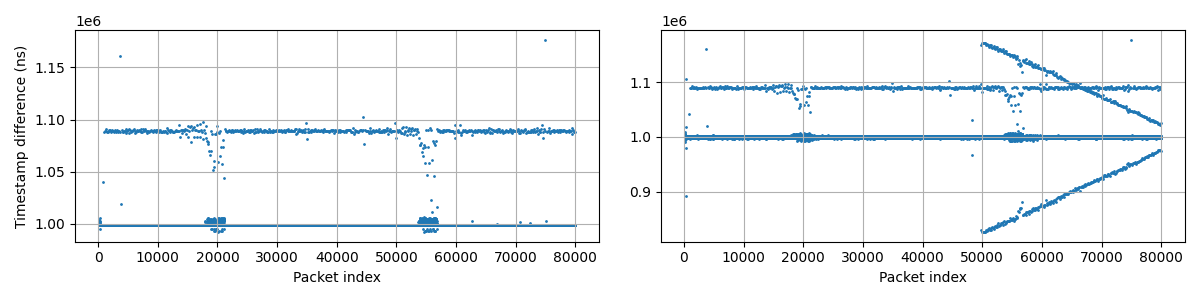
\includegraphics[width=\textwidth]{fig/xsk_80k_999us_powermax_4.png}
    \caption{Sending interval: $999\mu s$, method: AF\_XDP.}
    \label{fig:999us}
\end{subfigure}
\hfill
\begin{subfigure}{\textwidth}
    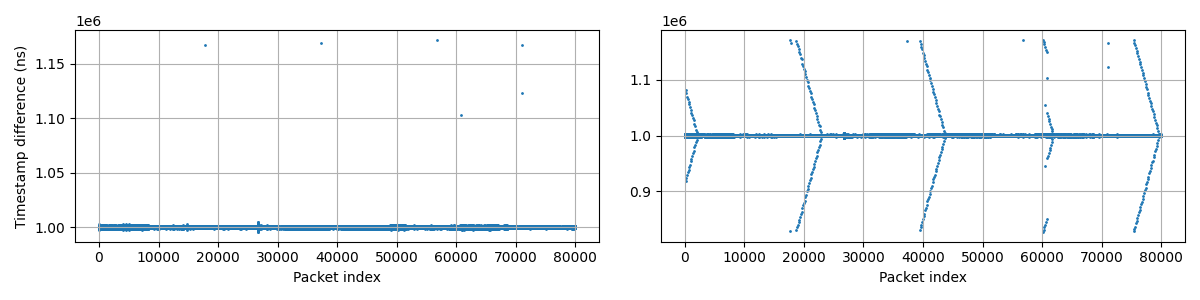
\includegraphics[width=\textwidth]{fig/fide_80k_1000us.png}
    \caption{Sending interval: $1000\mu s$, method: XDP offload. CPU isolation,
    interrupt shielding and no interrupt coalescence are applied in this 
    benchmark}
    \label{fig:1000us}
\end{subfigure}
\hfill
\begin{subfigure}{\textwidth}
  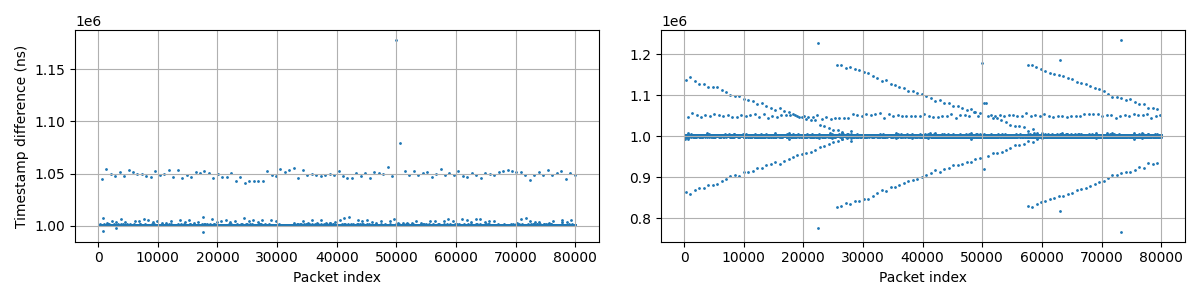
\includegraphics[width=\textwidth]{fig/xsk_80k_1001us_powermax.png}
  \caption{Sending interval: $1001\mu s$, method: RDMA.}
  \label{fig:1001us}
\end{subfigure}
\hfill
\begin{subfigure}{\textwidth}
  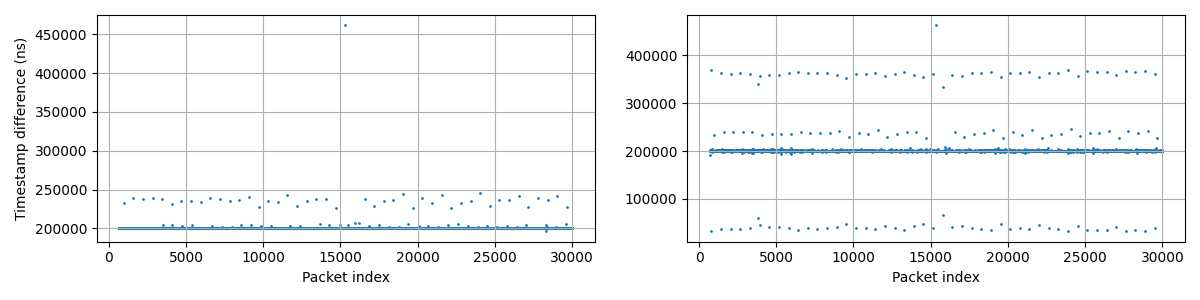
\includegraphics[width=\textwidth]{fig/xsk_30k_200us_powermax.png}
  \caption{Sending interval: $200\mu s$, method: AF\_XDP.}
  \label{fig:200us}
\end{subfigure}
\hfill
\begin{subfigure}{\textwidth}
  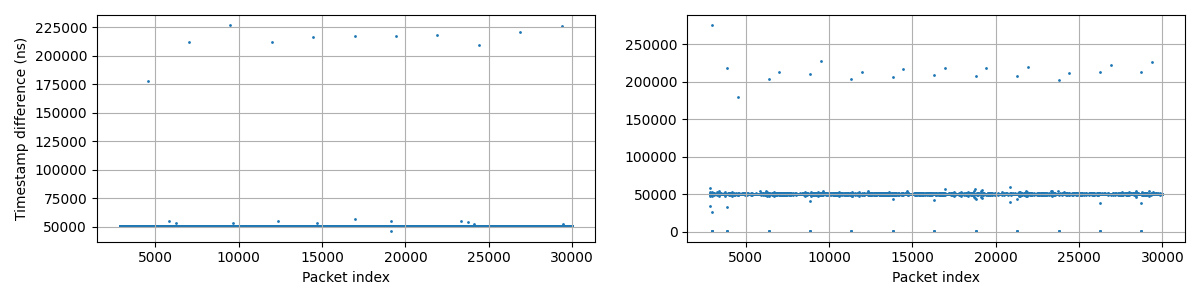
\includegraphics[width=\textwidth]{fig/xsk_30k_50us_powermax.png}
  \caption{Sending interval: $50\mu s$, method: AF\_XDP.}
  \label{fig:50us}
\end{subfigure}
\hfill  

\caption{Different examples of periodic outliers types \textbf{$ts_1$-offset} 
and \textbf{$ts_2$-arrow} observed with varying sending intervals and different
implementation methods. All tests were run with CPU cores at max frequency 
(C0 state)}
\label{fig:interval_variations}
\end{figure}

\subsection{Possible causes and observations}
Below we draft a list of possible causes and observations in Q\&A format in order
to outline what we have already tried to find the root cause of the outliers.
% \\
% \\
% \noindent
% \begin{tabularx}{0.9\textwidth} { 
%   | >{\raggedright\arraybackslash}X 
%   | >{\raggedright\arraybackslash}X 
%   | }
%   \hline
%   \textbf{Question} & \textbf{Observation} \\
%   \hline
%   Are the   & item 22  \\
%   \hline
% \end{tabularx}

\paragraph*{Are the peaks related to a particular bypass or software method?}
No, both peak types show with all RDMA, XDP and normal network stack. For 
instance, \autoref{fig:1000us} was tested with all implementations and leads
to the same pattern. 

\paragraph*{OS jitter interrupts, context switching etc. ?}
We ran experiments by reserving a number of cores exclusively for our programs, 
shielding such cores from interrupts, using the \texttt{isolcpus}, 
\texttt{nohz} kernel boot settings; we disable C-states, setting the CPU
power to the max. The full settings can be found in the \href
{https://github.com/swystems/det-bypass/blob/scale-ic-test/ansible/isolation.yaml}
{project repository}. These settings improve the overall latency and reduce the
number of random outliers but do not eliminate the periodic outlier types.

\paragraph*{Interrupts coalescence?}
No, the tests were performed with the interrupt coalescence settings of both
NICs disabled. 

\paragraph*{Code-related issue?}
Very unlikely. We test with 3 different programs. The send loop is just a busy 
loop pinned to a dedicated uninterrupted core. The simplest logic on the PONG
host is a XDP hosts that takes a timestamp as soon as a packet arrives,
inserts in the packet and sends it back. This executes as early as possible in
the network stack, right after the call to the driver. This means that 
the \textbf{$ts_2$-arrow} effect occurs before we can take any action.

\paragraph*{Caused by the network?}
\textbf{$ts_1$-offset} occurs before the packet is actually sent out, so 
the network can be excluded for it. It could play a role in 
\textbf{$ts_2$-arrow}, however CloudLab (our test cluster) guarantees
experiment reproducibility -- it is unlikely that concurrent traffic is 
present. Side effect of switching?

\paragraph*{Why do the outliers show in the PING transfer and never in PONG?}
If \textbf{$ts_2$-arrow} is related to packet reception / processing, we 
should observe it also at reception of the PONG packet, but this is not the case.
One explanation could be that \textbf{$ts_2$-arrow} is somehow caused by
\textbf{$ts_1$-offset}, hence related to the sending loop which happens only
at the beginning. However, no clear cause-effect has been identified up to now.  

\paragraph*{Unmaskable timing interrupts?}
Some kernel interrupts are unmaskable and they could explain outlier 
periodicity. However, they would not explain why the period changes according
to the sending interval.

\paragraph*{Memory effects?}
Paging, TLB / cache misses can introduce delays that can appear as periodic if 
we repeat the same action in a loop and use same size data structures as we do.
However, it is harder to justify the relationship between the sending interval 
and the outliers. Take for example \autoref{fig:1000us} and 
\autoref{fig:1001us}: a change of $1\mu s$ in the sending period causes
$>10\times$ more outliers - how would it relate to memory effects?

\paragraph*{Settings related to the specific NIC/driver?}
This seems to be one of the most likely causes. Further tests with an Intel X520-DA2 NIC
(see `notebook.ipynb`) and previous experiments with same NIC but different setup
show different kind of outliers and patterns. 

\end{document}